\chapter[Materials and Methods]{Materials and Methods}
\label{Materials}

This chapter details the materials and methods used in our
study. Specifically, we will cover the dataset, the model based on
CatBoost using graph-derived features, and our approach using Graph
Attention Networks (GATs) for predictive modeling. Our dataset
includes a range of meteorological, geographical, and flight
variables.

Our objective is to detail and model how to predict if a given
aircraft is going to delay due to holding maneuver in a supervised
learning setting.

\section{Datasets}
\label{Datasets}

The study utilizes two distinct datasets, each containing 42,336
observations, with identical meteorological, geographical, and
flight-related features. These datasets were constructed from a
combination of METAR and METAF weather reports, airport and flight
specifications sourced from ICEA. Each dataset serves a different
predictive modeling purpose—binary classification and regression—and
includes tailored labels to reflect these objectives

One of the primary challenges in the classification dataset is its
class imbalance, which could impact model performance. Common
approaches to address imbalance, such as oversampling or
undersampling, have been shown to introduce limitations like
overfitting and poor generalization (\cite{zhao2021graphsmote}, Graph
SMOTE). For graph machine learning tasks, oversampling is generally
problematic due to the risk of introducing artificial connectivity
patterns, while undersampling can lead to loss of critical structural
information. Therefore, we opted to explore model-based techniques
without applying these rebalancing methods.

\subsection{Binary Classification Dataset} The binary classification
dataset is used to predict the likelihood of a holding maneuver
occurring for a given flight. In this dataset, the label is a binary
value:
\begin{itemize}
    \item \textbf{Class 0 (No Holding)}: Represents flights with no
    holding delays, comprising 41,616 samples.
    \item \textbf{Class 1 (Holding)}: Indicates flights with holding
    delays, comprising only 720 samples.
\end{itemize} This significant imbalance between the classes adds
complexity to the classification task, as the model needs to
accurately predict a rare event within the data.

\subsection{Regression Dataset} The regression dataset aims to predict
the exact duration of holding delays in seconds, thus providing a
continuous label for each observation:
\begin{itemize}
    \item \textbf{Holding Time (Seconds)}: For this dataset, each
    holding event is represented by a floating-point number indicating
    the holding time in seconds. This approach enables a finer-grained
    analysis and can potentially improve operational insights by
    quantifying delay duration rather than merely classifying its
    occurrence.
\end{itemize}


\subsection{Meteorological Features} The dataset includes a
comprehensive range of meteorological variables from both METAR and
METAF reports:

\begin{itemize}
    \item \textbf{Wind Direction:} \texttt{metar\_wind\_direction},
    \texttt{metaf\_wind\_direction}
    \item \textbf{Wind Speed:} \texttt{metar\_wind\_speed},
    \texttt{metaf\_wind\_speed}
    \item \textbf{Wind Gusts:} \texttt{metar\_wind\_gust},
    \texttt{metaf\_wind\_gust}
    \item \textbf{Visibility:} \texttt{metar\_visibility},
    \texttt{metaf\_visibility}
    \item \textbf{Cloud Coverage:} \texttt{metar\_cloudcover},
    \texttt{metaf\_cloudcover}
    \item \textbf{Temperature:} \texttt{metar\_temperature},
    \texttt{metaf\_temperature}
    \item \textbf{Dew Point:} \texttt{metar\_dewpoint},
    \texttt{metaf\_dewpoint}
    \item \textbf{Altitude:} \texttt{metar\_elevation},
    \texttt{metaf\_elevation}
    \item \textbf{Sky Levels:} \texttt{metar\_skylev1},
    \texttt{metar\_skylev2}, \texttt{metar\_skylev3},
    \texttt{metar\_skylev4}, \texttt{metaf\_skylev1},
    \texttt{metaf\_skylev2}, \texttt{metaf\_skylev3},
    \texttt{metaf\_skylev4}
    \item \textbf{Altimeter Setting:} \texttt{metar\_altimeter},
    \texttt{metaf\_altimeter}
    \item \textbf{Weather Symbols:}
    \texttt{metar\_current\_wx1\_symbol},
    \texttt{metar\_current\_wx2\_symbol},
    \texttt{metar\_current\_wx3\_symbol},
    \texttt{metaf\_current\_wx1\_symbol},
    \texttt{metaf\_current\_wx2\_symbol},
    \texttt{metaf\_current\_wx3\_symbol}
\end{itemize}

\subsection{Geographical Features} The geographical features include
variables based on flight paths and airport information:

\begin{itemize}
    \item \textbf{Flight Distance:} Calculated as the geodesic
    distance between departure and arrival airports.
    \item \textbf{Airport Altitude:} \texttt{departure\_altitude} and
    \texttt{arrival\_altitude}, reflecting the elevation of the
    airports.
    \item \textbf{Latitude and Longitude:}
    \texttt{departure\_latitude}, \texttt{departure\_longitude},
    \texttt{arrival\_latitude}, and \texttt{arrival\_longitude} for
    geolocation-based analysis.
\end{itemize}

\subsection{Flight-Specific Features} These features capture specific
characteristics related to the flight and any runway head changes:

\begin{itemize}
    \item \textbf{Previous Runway Head Change:}
    \texttt{prev\_troca\_cabeceira}
    \item \textbf{Runway Head Change in Previous Hour:}
    \texttt{troca\_cabeceira\_hora\_anterior}
    \item \textbf{Flight Hour:} \texttt{hora\_do\_voo}
\end{itemize}

\section{CatBoost with Graph Features}
\label{sec:catboost_model}

This study employs the CatBoost model, a high-performance gradient boosting library, chosen specifically for its ability to handle categorical features and class imbalance effectively, as well as for its robust handling of noisy data \cite{prokhorenkova2018catboost}. CatBoost has been widely recognized for its superior performance in structured data problems, particularly when compared to other boosting algorithms like XGBoost and LightGBM, thanks to its unique techniques such as ordered boosting and categorical feature encoding. These innovations help prevent overfitting and enhance generalization in class unbalanced problems.

Here, we describe how CatBoost is combined the graph-based features that are extracted of our modeled airports network. These features are derived from the weighted directed graph and enconded as tabular features that are used as input to the model as we describe in the following sections.


\subsection{Graph Representation of the Flight Network}

\begin{figure}[h]
    \centering
    \begin{tikzpicture}[
        ->, % directed edges
        >=stealth, % arrow tip
        node distance=3cm, % distance between nodes
        airport/.style={circle, draw, minimum size=2cm, font=\Large}, % style for airports
        flight/.style={font=\small} % style for flights
    ]
    
    % Nodes (Airports)
    \node[airport] (A) {SP \\ \faPlaneDeparture}; % São Paulo with departure icon
    \node[airport] (B) [right of=A] {RJ \\ \faPlaneDeparture}; % Rio de Janeiro with departure icon
    \node[airport] (C) [below of=A] {MG \\ \faPlaneDeparture}; % Minas Gerais with departure icon
    
    % Edges (Flights)
    \draw[->] (A) to node[flight, above] {\tikz[baseline]{\node[rotate=0]{\faPlane};}} (B); % Flight from SP to RJ, plane icon aligned (0 degrees)
    \draw[->] (B) to node[flight, right] {\tikz[baseline]{\node[rotate=220]{\faPlane};}} (C); % Flight from RJ to MG, plane icon rotated 270 degrees
    \draw[->] (C) to node[flight, left] {\tikz[baseline]{\node[rotate=96]{\faPlane};}} (A); % Flight from MG to SP, plane icon rotated 135 degrees
    
    \end{tikzpicture}
    \caption{Airports and Directed Flights}
\end{figure}
    

To model the interactions in flight data, we represented the problem as a directed graph, depicted in Figure~\ref{fig:flight_network_graph}, where each node represents an airport, here we represent as states of Brazil: SP (São Paulo), MG (Minas Gerais), RJ (Rio de Janeiro). In this network:
\begin{itemize}
    \item Nodes represent airports.
    \item Directed edges represent flights, with each edge directed from the departure airport to the destination airport.
\end{itemize}
Given the frequent occurrence of multiple flights between the same pairs of airports (i.e., multiedges), we have in fact a multigraph, however we abstract it into a weighted directed graph as shown in \ref{fig:multigraph_to_weighted_graph}. Here, each edge's weight corresponds to the total number of flights between a specific pair of airports, transforming multiple directed edges into a single weighted edge. This abstraction allows us to calculate key network metrics more easily, which we then used as features in the CatBoost model.

\begin{figure}[h]
  \centering
  \begin{tikzpicture}[
    ->, % directed edges
    >=stealth, % arrow tip style
    node distance=4cm, % distance between nodes
    airport/.style={circle, draw, minimum size=2cm, font=\Large}, % style for airports
    flight/.style={font=\small, scale=0.8} % smaller size for flights
    ]

    % Multigraph (Left Side)
    \node[airport] (A1) {SP \\ \faPlaneDeparture}; % São Paulo with departure icon
    \node[airport] (B1) [right of=A1] {RJ \\ \faPlaneDeparture}; % Rio de Janeiro with departure icon
    \node[airport] (C1) [below of=A1, yshift=-1cm] {MG \\ \faPlaneDeparture}; % Minas Gerais with departure icon

    % Multiple flights in the multigraph (non-intersecting paths)
    \draw[->] (A1) to[bend left=20] node[flight, near start] {\tikz[baseline]{\node[rotate=0, scale=0.7]{\faPlane};}} (B1); % Flight 1 from SP to RJ
    \draw[->] (A1) to[bend left=40] node[flight, near start] {\tikz[baseline]{\node[rotate=0, scale=0.7]{\faPlane};}} (B1); % Flight 2 from SP to RJ
    \draw[->] (A1) to[bend left=60] node[flight, near start] {\tikz[baseline]{\node[rotate=0, scale=0.7]{\faPlane};}} (B1); % Flight 3 from SP to RJ

    \draw[->] (B1) to[bend right=20] node[flight, near start] {\tikz[baseline]{\node[rotate=270, scale=0.7]{\faPlane};}} (C1); % Flight 1 from RJ to MG
    \draw[->] (B1) to[bend right=40] node[flight, near start] {\tikz[baseline]{\node[rotate=270, scale=0.7]{\faPlane};}} (C1); % Flight 2 from RJ to MG

    \draw[->] (C1) to[bend right=20] node[flight, near start] {\tikz[baseline]{\node[rotate=135, scale=0.7]{\faPlane};}} (A1); % Flight 1 from MG to SP
    \draw[->] (C1) to[bend right=40] node[flight, near start] {\tikz[baseline]{\node[rotate=135, scale=0.7]{\faPlane};}} (A1); % Flight 2 from MG to SP
    \draw[->] (C1) to[bend right=60] node[flight, near start] {\tikz[baseline]{\node[rotate=135, scale=0.7]{\faPlane};}} (A1); % Flight 3 from MG to SP

    % Transformation arrow
    \node at ($(A1)!0.5!(B1)+(3.5,-2)$) {\Huge $\Rightarrow$};

    % Weighted Graph (Right Side)
    \node[airport] (A2) [right=6cm of A1] {SP \\ \faPlaneDeparture}; % São Paulo airport (weighted graph)
    \node[airport] (B2) [right of=A2] {RJ \\ \faPlaneDeparture}; % Rio de Janeiro airport (weighted graph)
    \node[airport] (C2) [below of=A2, yshift=-1cm] {MG \\ \faPlaneDeparture}; % Minas Gerais airport (weighted graph)

    % Weighted edges (single paths)
    \draw[->] (A2) to[bend left=20] node[flight, near end, yshift=0.3cm] { $W = 3$ \;} (B2); % Weighted edge from SP to RJ
    \draw[->] (B2) to[bend right=20] node[flight, near end, xshift=0.2cm] {\; \;\;\;\;\; \; $W = 2$  } (C2); % Weighted edge from RJ to MG
    \draw[->] (C2) to[bend right=20] node[flight, near end, xshift=-0.8cm] {  $W=3$  } (A2); % Weighted edge from MG to SP

  \end{tikzpicture}
  \caption{Transformation of a multigraph of flights into a weighted directed graph. The multigraph (left) represents multiple flights between airports. In the weighted graph (right), edges are aggregated to show total flights as weights.}
  \label{fig:multigraph_to_weighted_graph}
\end{figure}





\subsection{Graph-based Features}
The graph-based features encode essential structural information about the flight network, capturing connectivity, centrality, and robustness. These features are crucial for understanding the influence of each airport within the network and its potential impact on flight holding patterns. 

However, this is not a trivial task, as the graph-based features are not directly compatible with the model. Although we have already made this simplification of the multigraph, transforming it into a weighted directed graph, we still need to extract the features from the graph and encode them as tabular data. 

However, the modelling will impact dramatically in the resulting graph-based features. For instance, we need to calculate edge measures, but this is not so explored as node measures, so the lack of possibilities is a challenge to be overcome.  Another challenge is the direction, that is, we have to create edge measures in a directed weighted graph, which is hard, as we detailed in section \ref{classical_learning}, because most of the complex networks measures proposed are `node centric' and for undirected graphs.

With this in mind, we can observe why the weighted graph transformation was so important, since the measures available for our setting are strongly dependent to the weight (as we will detail later), and our graph is almost totally connected, so in undirected unweighted setting they would be approximately equal, leaving no information. The following graph metrics were calculated from the weighted directed graph:

\begin{itemize}
    \item \textbf{Betweenness Centrality:} Captures the relative importance of each airport in terms of the routes it controls within the network. Higher values indicate airports that serve as critical transit points.
    \item \textbf{Flow Betweenness:} Highlights the flow dynamics of connections, showing how flights tend to route through certain airports, which may correlate with congestion.
    \item \textbf{Edge Connectivity:} Indicates the robustness of airport connections, with higher values signifying more resilient routes between airports that could better handle rerouting needs.
    \item \textbf{Degree Difference:} Measures the disparity between in-degrees and out-degrees at each node, helping to identify key hubs or spokes in the network.
    \item \textbf{Google Matrix:} Based on PageRank centrality, the Google matrix provides a probabilistic transition representation for each airport, which reflects both local and global connectivity.
\end{itemize}

As we can see, these features are not commonly used in the literature. Here is where the weighted network plays a crucial role, edge betweeness centrality \cite{newman2004finding} is constructed using shortest paths in the network, thus the weight will be crucial part of it, since without it the graph is almost fully connected, the shortest path will be almost the same for all pairs of nodes. The same happens with flow betweeness centrality \cite{brandes2001faster}, that is a measure of the amount of flow that goes through a node, and the weight will be crucial to calculate it. The edge connectivity \cite{tarjan1972depth} is a measure of the minimum number of edges that must be removed to disconnect the graph, and the weight will be crucial to calculate it. The degree difference is a measure of the difference between the in-degree and out-degree of a node, and the weight will be crucial to calculate it. The Google matrix is a measure of the importance of a node in the network, and the weight will be crucial to calculate it.

These features enhance the CatBoost model by embedding graph-theoretic insights into its predictive capabilities, ultimately enabling a more nuanced understanding of how network dynamics relate to flight holding patterns.


\section[Graph Attention Network]{Graph Attention Network}
\label{Graph Attention Network}

As we previously described, the GAT model in \ref{spatial-based} has a large range of applications, from drug discovery to fake news detection \cite{keywordsCaravanti}. The GAT model leverages the underlying graph structure but does not rely on explicitly computed graph-derived features like the CatBoost model does. Instead, it learns node representations in an end-to-end manner, enabling the model to capture the relationships between airports and flights directly from the data.

\input{img/gat_layer.tex}

\begin{figure}[h]
  \centering
  \begin{tikzpicture}
      % Define colors for different attention heads
      \definecolor{color1}{RGB}{60, 120, 216}  % Blue for Head 1
      \definecolor{color2}{RGB}{34, 139, 34}   % Green for Head 2
      \definecolor{color3}{RGB}{255, 99, 71}   % Red for Head 3
      
      % Define nodes
      \node[circle, draw, thick] (node1) at (0,0) {$\vec{h}_1$};
      \node[circle, draw, thick] (node2) at (5,0) {$\vec{h}_2$};
      
      % Flight 1 - Blue attention heads, no intersections
      \draw[-stealth, thick, color1!50] (node1) .. controls +(1,2) and +(-1,2) .. node[midway, above, color1!50] {$\alpha_{1,2}^{(1)}$} (node2);
      \draw[-stealth, thick, color1!70] (node1) .. controls +(1,1.5) and +(-1,1.5) .. node[midway, above, color1!70] {$\alpha_{1,2}^{(2)}$} (node2);
      \draw[-stealth, thick, color1] (node1) .. controls +(1,1) and +(-1,1) .. node[midway, above, color1] {$\alpha_{1,2}^{(3)}$} (node2);
      
      % Flight 2 - Green attention heads, spaced below Flight 1
      \draw[-stealth, thick, color2!50] (node1) .. controls +(1,-1) and +(-1,-1) .. node[midway, below, color2!50] {$\alpha_{1,2}^{(1)}$} (node2);
      \draw[-stealth, thick, color2!70] (node1) .. controls +(1,-1.5) and +(-1,-1.5) .. node[midway, below, color2!70] {$\alpha_{1,2}^{(2)}$} (node2);
      \draw[-stealth, thick, color2] (node1) .. controls +(1,-2) and +(-1,-2) .. node[midway, below, color2] {$\alpha_{1,2}^{(3)}$} (node2);

      % Flight 3 - Red attention heads, even lower to avoid overlap
      \draw[-stealth, thick, color3!50] (node1) .. controls +(1,-3) and +(-1,-3) .. node[midway, below, color3!50] {$\alpha_{1,2}^{(1)}$} (node2);
      \draw[-stealth, thick, color3!70] (node1) .. controls +(1,-3.5) and +(-1,-3.5) .. node[midway, below, color3!70] {$\alpha_{1,2}^{(2)}$} (node2);
      \draw[-stealth, thick, color3] (node1) .. controls +(1,-4) and +(-1,-4) .. node[midway, below, color3] {$\alpha_{1,2}^{(3)}$} (node2);

      % Output node
      \node[circle, draw, thick, right=7em of node2, opacity=0.8] (output) {$\vec{h}_2'$};
      
      % Aggregation line with label
      \draw[-stealth, thick, color1!70] (node2) -- ++(1.5,0) -- ++(1.5,0) node[midway, above, black] {concat/avg} -- (output);
  \end{tikzpicture}
  \caption{GAT Layer with multi-head attention for three different flights between nodes.}
  \label{fig:gat_layer}
\end{figure}

